\section{Methods}%
\label{sec:methods}

\subsection{Mobile Manipulator's Representation}

Let us consider a velocity controlled mobile manipulator consisting of a mobile base with a mounted robotic arm. The coupled system's dynamics are described by the discrete-time non-linear system
\begin{equation}
  \z_{k+1} = f(\z_k, \u_k), 
\end{equation}
where $\z_k$ and $\u_k$ describe the state and the control inputs at the time-step $k$, respectively. The robot's state is the base position and orientation, and the manipulator's joint positions, $\z = [x,y,\theta,\mathbf{q}^{\textrm{arm}}]$. The robot's control inputs are the left $u^l$ and right $u^r$ wheel velocity, and joint velocities $\dot{\mathbf{q}}^{\textrm{arm}}$, hence $\mathbf{u}=[u^l,u^r,\dot{\mathbf{q}}^{\textrm{arm}}]$.  We denote $\mathcal{Z}$ and $\mathcal{U}$ as the corresponding state and control commands admissible sets, respectively.
The space occupied by the robot is denoted as $\mathcal{B}(\z)=\bigcup_{i \in \{1,\dots,n_{\textrm{links}} \}}\mathcal{B}_i(\z)$ and $\mathcal{B}_i(\z)$ denotes the space occupied by the ~{$i$-th} robot's link with $i\in[0,N_{\textrm{links}}]$. We approximate the state occupied by each link by spheres with radius $r_i$. The space occupied by the static obstacles and dynamic obstacles is represented as $\mathcal{O}^{\textrm{static}}$ and $\mathcal{O}^{\textrm{dynamic}}$, respectively. To limit the complexity of the problem we only consider a limited number $n_{\textrm{links}} \le N_{\textrm{links}}$ of the robot's links and the $n_{\textrm{dyn}} $ closest dynamic obstacles.

\subsection{Mobile Manipulator's Model}%
\label{sub:transition_function}
%
 Here, we assume a differential drive model for the base and first order dynamics for the robotic manipulator:
%The transition function for the presented robot is composed of a differential drivable mobile base and a velocity controlled robotic arm. We can write the dynamics of the system as
\begin{equation}
    \dot{\z} = \begin{bmatrix} \frac{1}{2}cos(\theta)(u^l + u^r) r_{\textrm{wheel}} \\
                                      \frac{1}{2}sin(\theta)(u^l + u^r) r_{\textrm{wheel}} \\
                                      \frac{(u^r - u^l)r_{\textrm{wheel}}}{L_{\textrm{wheel}}} \\
                                      \dot{\vec{q}}_{\textrm{arm}} \end{bmatrix}, 
\end{equation}
where $r_{\textrm{wheel}}$ and $L_{\textrm{wheel}}$ are the wheel radius and distance between the two controllable wheels, respectively. The discrete transition function $f(\z_k, \u_k)$ can be found using a discretization scheme (e.g. Backward-Euler or Runge-Kutta).
%where $\theta$ is the orientation of the base, $r_{\textrm{wheel}}$ and $L_{\textrm{wheel}}$ are the wheel radius and distance between the two controllable wheels, respectively. $u_1, u_2$ are the commanded velocities for the wheels and $\dot{\vec{q}}_{\textrm{arm}}$ is the commanded joint velocity vector for the robotic arm.
%To ensure collision-free motion, we explicitly define a set of constraints. 
The set of admissible states ($\mathcal{Z}$) and control inputs ($\mathcal{U}$) is defined by the joint position and velocity limits
\begin{equation}
  \begin{split}
    \vec{q_{\textrm{min}}} \leq \vec{q_{\textrm{arm}}} \leq \vec{q_{\textrm{max}}} \\ 
    \vec{u_{\textrm{min}}} \leq \vec{u_{\textrm{wheels}}} \leq \vec{u_{\textrm{max}}} \\
    \vec{\dot{q}_{\textrm{min}}} \leq \vec{\dot{q}_{\textrm{arm}}} \leq \vec{\dot{q}_{\textrm{max}}}.
\end{split}
\end{equation}
where $\vq_{\textrm{min}}$ and $\vq_{\textrm{max}}$, $\vu_{\textrm{min}}$ and $\vu_{\textrm{max}}$ and, $\dot{\vq}_{\textrm{min}}$ and $\dot{\vq}_{\textrm{max}}$ are the minimum and maximum joint position position, wheel velocity limits and joint velocity limits, respectively.

\subsection{Optimization Problem}%
\label{sub:optimization_problem}
Consider that a reference path in $\mathbb{R}^2$ is provided for the base, denoted as a sequence of $M$ waypoints, $([x,y]_m)_{m=0}^M$. The goal is to generate feasible control commands for the whole mobile manipulator enabling it to track the provided path while avoiding collisions in 3D space with dynamic and static obstacles. 
%In this paper, we assume that a global path for the base's motion is available and can be denoted as a sequence of $K$ waypoints, $([x,y]_k)_{k=0}^K$. To create a continuous path's representation, we approximate the provided path using a cubic \textit{Bézier Curve} and use a normalized time parametrization, $\phi \in [0, 1]$, and where $\vec{p}^{r}_{t} = [x,y]^{r}_{t}$ is the desired base position at time-step $t$. The desired base orientation, $\theta^{r}_t$, is defined as the curve's tangent.  
Hence, we formulate the trajectory planning problem for the unified system, base plus arm, as an optimization problem. As a result, we can explicitly formulate collision avoidance and kinodynamic constraints and compute control commands to generate feasible and collision-free motions.
The optimization problem is formulated as
%
\begin{subequations}
\begin{alignat}{1}
\label{eq:cost_function} J^{\star} = &\min_{\z_{0:N}, \u_{0:N}} \sum_{k=0}^{N} J(\z_k,\u_k), \\
\label{eq:dynamics} s.t. \quad &\z_{k+1} = f(\z_k, \u_k) \quad \forall k < N,  \\
\label{eq:coll_constraints}           &\mathcal{B}(\z_k) \cap\left(\mathcal{O}^{\textrm{static}} \cup
            \mathcal{O}^{\textrm{dynamic}}\right) = \emptyset, \\
\label{eq:state_constraints} &\u_k \in \mathcal{U}, \z_k \in \mathcal{Z},\\
\label{eq:initial_conditions} &\z_0 = \z(0).
\end{alignat}
\end{subequations}
%
In this formulation, Eq.~\ref{eq:cost_function} is the cost function (Section \ref{sub:cost_function}), Eq.~\ref{eq:dynamics} represents the
kinodynamic constraints of the system (Section \ref{sub:transition_function}), Eq.~\ref{eq:coll_constraints}
formalizes collision avoidance with static (Section \ref{sub:collision_avoidance_static}) and dynamic obstacles (Section \ref{sub:collision_avoidance_dynamic}), and Eq.~\ref{eq:state_constraints} defines the set of admissible
states and control inputs (Section \ref{sub:transition_function}). Finally, Eq.~\ref{eq:initial_conditions} defines the initial state conditions. Note that we optimize over a prediction horizon $N$ allowing to avoid dynamic obstacles in advance.


\subsection{Cost Function}%
\label{sub:cost_function}
To track the reference path, we first create a continuous path representation by approximating the provided reference path using a cubic \textit{Bézier Curve} and using a normalized time parametrization, $\phi_k \in [0, 1]$. We denote $\vec{p}_k$ and $\theta_k$ as the predicted base position and orientation at time step $k$ and $\vec{p}^{r}_{k}(\phi_k) = [x,y]^{r}_{k}$ and $\theta_k^r(\phi_k)$ as the reference base position and orientation at future time-step $k$, respectively.
Then, we define a tracking error vector $\boldsymbol{e}_k := [e^c(\boldsymbol{z}_k,\phi_k),e^l(\boldsymbol{z}_k,\phi_k)]^\textrm{T}$ composed by the contour $e^c(\boldsymbol{z}_k,\phi_k)$ and a lag-error $e^l(\boldsymbol{z}_k,\phi_k)$, and computed as it follows

\begin{equation}
  \vec{e}_{k} =
      \begin{bmatrix}
        cos(\theta_k^r) & sin(\theta^r_k) \\
        -sin(\theta^r_k) & cos(\theta^r_k)
      \end{bmatrix} 
    \left(\vec{p}^{\textrm{r}}_{k} - \vec{p}_{k}\right).
\end{equation}
%
The cost function $J(\z_{k}, \u_{k})$ is composed of the weighted ($W_\ve$) quadratic tracking error, the weighted ($W_\vq$) arm configuration distance-to-goal and the weighted ($W_\vu$) quadratic inputs to penalize high control commands . The difference between the current and desired orientation is quadratically weighted to ensure that the robot is moving forward ($w_{\theta}$).
 In addition, to relax the problem, we introduce the slack variable $s$ and penalize its weighted norm
\begin{equation}
  \begin{aligned}
  J(\z_{k}, \u_{k}) &
    = \norm{\ve_{k}}_{W_\ve} +\norm{ \vec{u}_k}_{W_\vu}  + \norm{\left(\theta^r_{k} - \theta_k\right)}_{w_{\theta}} \\
    & + \norm{\vec{q}_k - \vec{q}_{\textrm{des,k}}}_{W_q} 
    + \norm{s_k}_{w_{\textrm{slack}}}.
  \end{aligned}
\end{equation}

\subsection{Collision Avoidance For Static Obstacles}%
\label{sub:collision_avoidance_static}

In this paper, we tackle the problem of avoiding static obstacles in 3D space. Hence, we employ an octree representation of the static obstacles fed directly from 3D sensor data (e.g., depth camera). %The octree is constantly updated based on the perception of the environment.
%
%\textit{Convex Regions}
Given this information, we propose to model the free space as a set of convex polyhedrons around the robot's links instead of explicitly describing individual obstacles. This representation allows us to limit the number of collision constraints regardless of the number of obstacles, and depending only on the number of robot's links and the number of planes used for the convex regions. To compute the convex regions, we employ the method proposed in \cite{Liu2017} using an ellipsoid based regional inflation.
%to find this regions.
\begin{figure}[h]
  \centering
  \begin{subfigure}[b]{0.5\linewidth}
    \centering
    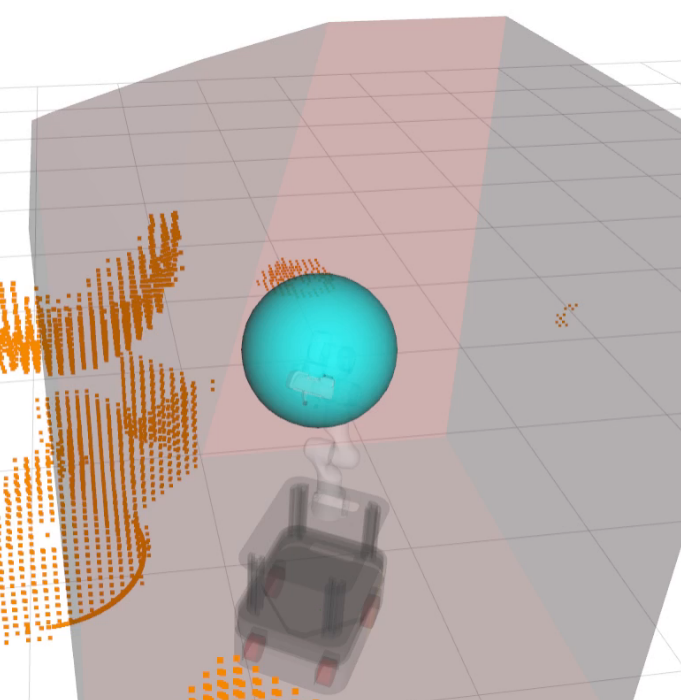
\includegraphics[height=0.7\linewidth]{methods/sphere_polyhedron.png}
    \caption{Polyhedron}
  \end{subfigure}
  \begin{subfigure}[b]{0.45\linewidth}
    \centering
    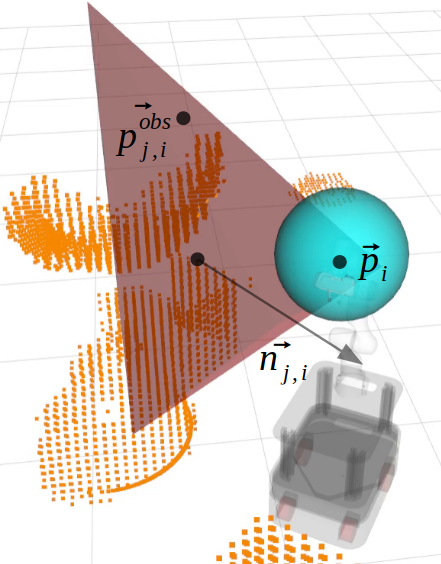
\includegraphics[height=0.7\linewidth]{methods/sphere_dist.png}
    \caption{Single Inequality}
  \end{subfigure}
  \caption{Generated polyhedron representing the free space in the presence of sensed pointcloud (orange) for last link and the corresponding sphere on the robot (blue) and visualization sphere-plane inequality constraint (right).}%
  \label{fig:plane_sphere}
\end{figure}
%
Fig.~\ref{fig:plane_sphere} depicts an example of one of these convex regions computed for one robot's link.
For each $i\in [1,n_{\textrm{links}}]$, we compute a polyhedron with $n_{\textrm{planes}}$ planes representing the free-space around the $i$-th link. 

Then, we impose a linear inequality constraint between each $j$-th polyhedron plane and $i$-th link to ensure $\mathcal{B}(\z_k) \cap \mathcal{O}^{\textrm{static}} = \emptyset$ as
%
\begin{equation}
    \begin{split} 
        & \va^T \vp_i\le b - (r_i + d_{\textrm{safety}}) \\ &\forall i \in \{1,\dots,n_{\textrm{links}}\} , \,\,\,\,
        \forall j \in \{1,\dots,n_{\textrm{planes}}\},
    \end{split}
\end{equation}
with $\va = \vn_{j,i}$ and $b = -\vn_{j,i}^T\vp^{\textrm{obs}}_{j,i}$, where $\vn_{j,i}$ is the normal vector and $\vp^{\textrm{obs}}_{j,i}$ a point on the $j$-th polyhedron's plane enclosing the ~{$i$-th} robot link, $\vp_i$ is the $i$-th link position, and $d_{\textrm{safety}}$ an hyper-parameter that acts as a safety margin. The proposed collision constraint ensures that each link's space is inside the convex region and thus free of static obstacles, as depicted in Fig.\ref{fig:plane_sphere}.
%
\subsection{Collision Avoidance For Moving Obstacles}%
\label{sub:collision_avoidance_dynamic}
%
To avoid moving obstacles, it is necessary to propagate the states of the dynamic obstacles over the planning horizon $N$. Using the previous constraint for dynamic collision avoidance requires the propagation of the 3D octree and the computation of the convex polyhedra for every stage, which is highly computationally expensive. 

Hence, we propose to model dynamic obstacles as spheres. For each dynamic obstacle $d$ we assume to know the position 
$\vec{p}^{\textrm{dyn}}_{d}$, velocity $\vv_{d}^{\textrm{dyn}}$, and radius $r_d^{\textrm{dyn}}$, with $d=\{1,\dots,n_{\textrm{dyn}}\}$. Then, we employ a constant velocity model to obtain predictions on the dynamic obstacle's future positions, $\bar{\vec{p}}^{\textrm{dyn}}_{d,k} = \vec{p}_{d}^{\textrm{dyn}} + k\Delta t\vec{v}_{d}^{\textrm{dyn}}$.
Finally, we define a non-linear collision avoidance constraint ensuring that the obstacle's space does not intersect with any link's space, %Using this prediction, we can formulate collosion avoidance with dynamic 
$\mathcal{B}_i(\z_k) \cap\mathcal{O}^{\textrm{dynamic}}=\emptyset \,\, \forall i \in [1,n_{\textrm{links}}]$, imposing that the distance between both bounding spaces is larger than the sum of their radius and the previously introduced safety margin
%obstacle over the time horizon $N$ as a sphere-sphere constraint.
\begin{equation}
  \begin{split}
  &\norm{\bar{\vec{p}}_{d,k}^{\textrm{dyn}} - \vp_{i,k}}  
    \geq r_d^{\textrm{dyn}} + r_i + d_{\textrm{safety}}  \\ &\forall i \in\{1,\dots,n_{\textrm{links}}\},\; d\in\{1,...,n_{dyn}\},\;k\in{0,...,N},
  \end{split}
\end{equation}
where $\vp_{i}$ is the position of the $i$-th robot link and $r_d^{\textrm{dyn}}$ the $d$-th dynamic obstacle radius.


